%
% diskretisierung.tex
%
% (c) 2020 Prof Dr Andreas Müller, Hochschule Rapperswil
%
\begin{frame}
\frametitle{Diskretisation}
\vspace{-15pt}
%
\begin{columns}[t]
\begin{column}{0.48\hsize}
\begin{block}{Gitterpunkte}
Funktion $u(x,y)$ ersetzen durch Werte 
$u_{ij}=u(x_i,y_j)$ in Gitterpunkten
\end{block}
\end{column}
\begin{column}{0.48\hsize}
\uncover<2->{%
\begin{block}{Volumina}
Funktion $u(x,y)$ ersetzen durch repräsentative Werte $u_{ij}$ über Volumina,
z.~B.~Integrale von $u(x,y)$
\end{block}}
\end{column}
\end{columns}
%
\begin{columns}[t]
\begin{column}{0.48\hsize}
\begin{center}
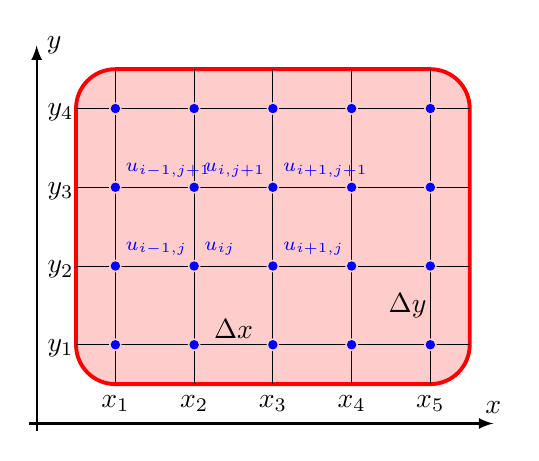
\begin{tikzpicture}[>=latex,thick]

\fill[color=red!20]
        (1.0,0.5)
        -- (5.0,0.5) to[out=0,in=-90]   (5.5,1.0)
        -- (5.5,4.0) to[out=90,in=0]    (5.0,4.5)
        -- (1.0,4.5) to[out=180,in=90]  (0.5,4.0)
        -- (0.5,1.0) to[out=-90,in=180] (1.0,0.5) -- cycle;

\draw[color=red,line width=1.4pt]
        (1.0,0.5)
        -- (5.0,0.5) to[out=0,in=-90]   (5.5,1.0)
        -- (5.5,4.0) to[out=90,in=0]    (5.0,4.5)
        -- (1.0,4.5) to[out=180,in=90]  (0.5,4.0)
        -- (0.5,1.0) to[out=-90,in=180] (1.0,0.5) -- cycle;

\foreach \x in {1,...,5}{
	\draw[line width=0.3pt] (\x,0.5) -- (\x,4.5);
	\node at (\x,0.6) [below] {$x_\x\mathstrut$};
}
\foreach \y in {1,...,4}{
	\draw[line width=0.3pt] (0.5,\y) -- (5.5,\y);
	\node at (0.6,\y) [left] {$y_\y\mathstrut$};
}

\foreach \x in {1,...,5}{
	\foreach \y in {1,...,4}{
		\fill[color=red!20] (\x,\y) circle[radius=0.08];
		\fill[color=blue] (\x,\y) circle[radius=0.06];
	}
}
\node[color=blue] at (1,2) [above right] {$\scriptstyle u_{i-1,j}$};
\node[color=blue] at (2,2) [above right] {$\scriptstyle u_{ij}$};
\node[color=blue] at (3,2) [above right] {$\scriptstyle u_{i+1,j}$};
\node[color=blue] at (1,3) [above right] {$\scriptstyle u_{i-1,j+1}$};
\node[color=blue] at (2,3) [above right] {$\scriptstyle u_{i,j+1}$};
\node[color=blue] at (3,3) [above right] {$\scriptstyle u_{i+1,j+1}$};

\node at (2.5,{1-0.05}) [above] {$\Delta x$};
\node at ({5+0.08},1.5) [left] {$\Delta y$};

\draw[->] (-0.1,0)--(5.8,0) coordinate[label={$x$}];
\draw[->] (0,-0.1)--(0,4.8) coordinate[label={right:$y$}];

\end{tikzpicture}
\end{center}
\end{column}
\begin{column}{0.48\hsize}
\begin{center}
\uncover<2->{%
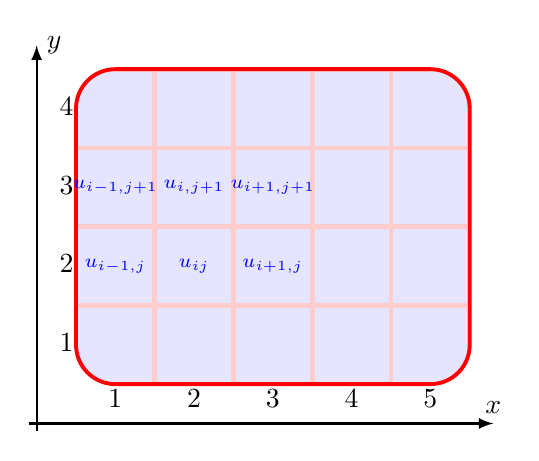
\begin{tikzpicture}[>=latex,thick]
\fill[color=red!20]
        (1.0,0.5)
        -- (5.0,0.5) to[out=0,in=-90]   (5.5,1.0)
        -- (5.5,4.0) to[out=90,in=0]    (5.0,4.5)
        -- (1.0,4.5) to[out=180,in=90]  (0.5,4.0)
        -- (0.5,1.0) to[out=-90,in=180] (1.0,0.5) -- cycle;

\foreach \x in {1,...,5}{
	\foreach \y in {1,...,4}{
		\fill[color=blue!10] ({\x-0.47},{\y-0.47}) rectangle ({\x+0.47},{\y+0.47});
	}
}

\fill[color=white]
        (1.0,0.5)
        -- (5.0,0.5) to[out=0,in=-90]   (5.5,1.0)
        -- (5.5,4.0) to[out=90,in=0]    (5.0,4.5)
        -- (1.0,4.5) to[out=180,in=90]  (0.5,4.0)
        -- (0.5,1.0) to[out=-90,in=180] (1.0,0.5)
	-- (0,0) -- (0,5) -- (6,5) -- (6,0) -- cycle;

\draw[color=red,line width=1.4pt]
        (1.0,0.5)
        -- (5.0,0.5) to[out=0,in=-90]   (5.5,1.0)
        -- (5.5,4.0) to[out=90,in=0]    (5.0,4.5)
        -- (1.0,4.5) to[out=180,in=90]  (0.5,4.0)
        -- (0.5,1.0) to[out=-90,in=180] (1.0,0.5) -- cycle;

\foreach \x in {1,...,5}{
	\node at (\x,0.6) [below] {$\x\mathstrut$};
}
\foreach \y in {1,...,4}{
	\node at (0.6,\y) [left] {$\y\mathstrut$};
}

\node[color=blue] at (1,2) {$\scriptstyle u_{i-1,j}$};
\node[color=blue] at (2,2) {$\scriptstyle u_{ij}$};
\node[color=blue] at (3,2) {$\scriptstyle u_{i+1,j}$};
\node[color=blue] at (1,3) {$\scriptstyle u_{i-1,j+1}$};
\node[color=blue] at (2,3) {$\scriptstyle u_{i,j+1}$};
\node[color=blue] at (3,3) {$\scriptstyle u_{i+1,j+1}$};

\draw[->] (-0.1,0)--(5.8,0) coordinate[label={$x$}];
\draw[->] (0,-0.1)--(0,4.8) coordinate[label={right:$y$}];

\end{tikzpicture}}
\end{center}
\end{column}
\end{columns}
\end{frame}
